\documentclass[fleqn,10pt]{physiome}
% Use option lineno for line numbers 

\articletype{Letter}
%% Choose from Original, Retrospective, Review, Letter

\title{Model of skeletal muscle cramp and its reversal}

\author[1][kazuyo.tasaki@dpag.ox.ac.uk]{Kazuyo Tasaki}
\author[1]{Penelope J. Noble}
\author[2]{Alan Garny}
\author[3]{Paul R. Shorten}
\author[2]{Nima Afshar}
\author[1][kazuyo.tasaki@dpag.ox.ac.uk denis.noble@dpag.ox.ac.uk]{Denis Noble}
\affil[1]{Department of Physiology, Anatomy \& Genetics, Medical Sciences Division, University of Oxford, United Kingdom}
\affil[2]{Auckland Bioengineering Institute, University of Auckland, New Zealand}
\affil[3]{Institute of Agricultural Research, New Zealand}

%% The following lines can be omitted when submitting;
%% information will be added by editors
\publicationdate{28 August 2020}
\editor{Karin Lundengård}
\curator{Anand Rampadarath}
\submitteddate{25 August 2020}
\accepteddate{25 August 2020}
\citethisas{Kazuyo et al. (2020)\\ Model of skeletal muscle cramp and its reversal. Physiome.}{10.36903/physiome.12871364}
\begin{document}

\maketitle

\begin{abstract}
In an other paper \citep{Noble2019Incorporation}, we developed the \cite{shorten2007mathematical} model of skeletal muscle by incorporating equations such as surface calcium fluxes. In further research in this paper, we succeeded in reproducing muscle cramp, as well as its prevention and reversal, by investigating muscle contraction and cramp, in which calcium regulatory networks are involved, using the extended model in comparison with the original model. Incorporation of data from a Traditional Medicine from root extracts of peony and licorice and one of its pure chemicals was modelled. Sensitivity analysis of the extended model shows the robustness of the calcium regulatory networks. Muscle cramp, in the extended model, requires calcium influx via the L-type calcium channel and it will not occur without calcium influx. Reduced calcium influx can delay or prevent cramp. Increased interstitial potassium is implicated in developing and maintaining cramp. Mechanism of reversal of cramp requires wash-out of extracellular potassium via increased blood flow, followed by calcium efflux via sodium-calcium exchange. This paper shows the first successful quantitative electrophysiological and mechanical model of cramp and of its reversal.
\end{abstract}

\keywords{Skeletal muscle model, muscle fatigue, muscle cramp, Ca$^{2+}$ \ influx, K$^+$ \ wash-out of, \  Ca$^{2+}$ \ efflux, \ Na$^+$- Ca$^{2+}$ \ exchanger.}

\primarypubs[10.36903/physiome.12871364]{References}{Noble2019Incorporation}

\section{Introduction}

\textit{Purpose of development of the original model}\\\newline
Both fatigue and cramp are important pathologies of skeletal muscle. The \cite{shorten2007mathematical} model reproduces muscle fatigue, but not muscle cramp. Yet, the latter is incapacitating and often painful. Without such a model, it is impossible to make or test predictions concerning the prevention or reversal of muscle cramp.\\\newline
The prevalence of muscle cramp in patients with muscle cramp over the age of 60 is around 46\% \citep{maisonneuve2016prevalence}, with a high impact on quality of life: 21\% of sufferers “described their symptoms as very distressing”. It is therefore a widespread health problem in aging populations. This data is for rest cramps  \citep{naylor1994general}. Exercise associated muscle cramps are also common with acute pain, and distress affecting performance that can last days \citep{millerexercise}. The authors note that “their cause remains unknown”.\\\newline
It is difficult to account for the development of muscle cramp without supposing that calcium influx may be important. Cramp may be defined as a maintained contraction that cannot be immediately reversed by ceasing to electrically excite the muscle. Overloading the muscle fibres with calcium might satisfy this criterion since it would maintain contraction for as long as the free intracellular calcium is above the threshold for activating the cross-bridge reactions of the contractile proteins.

\begin{figure}[h!]
\centering
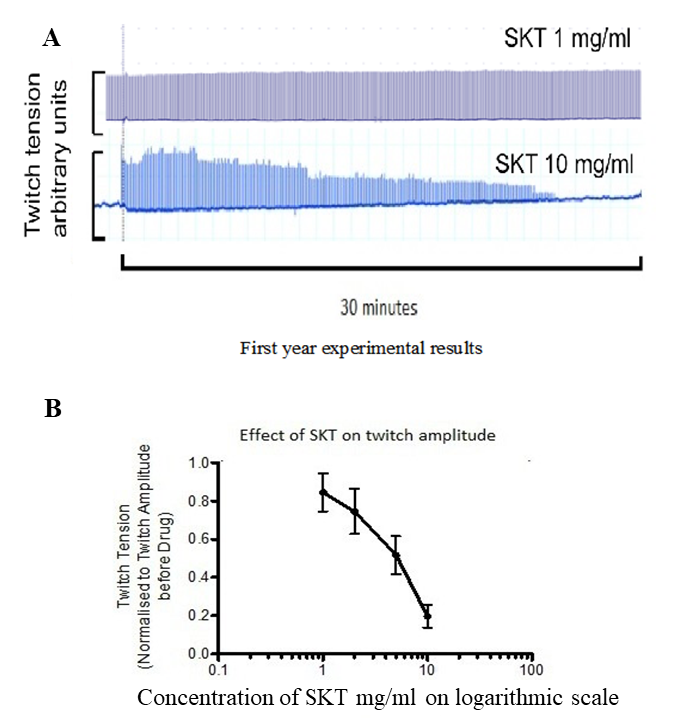
\includegraphics[width=0.65\linewidth]{figure01}
\caption{Actions of SKT in isolated diaphragm of guinea pigs in twitch amplitude at a frequency stimulation of 0.1 Hz.  
A: top trace:1 mg/ml SKT shows no action; bottom trace: 10 mg/ml SKT shows slow action.
B: dose-response relation of actions of SKT in isolated diaphragm of guinea pigs in twitch amplitude at a frequency stimulation of 0.1 Hz (from \citep{Sam2015Actions})}
\label{fig01}
\end{figure}
It is therefore important to incorporate surface membrane calcium fluxes in the Shorten model \citep{shorten2007mathematical}. As we have shown in the other paper \citep{Noble2019Incorporation}, our extensions of the model succeed in incorporating these fluxes, as well as those of extracellular potassium ions in exchange with bulk (plasma) potassium, [K]$_b$.

\section{Model description}

\textit{Supporting experimental data showing why sarcolemmal calcium transporters need to be incorporated}\\\newline
For interaction with this modelling research, we use some of the experimental data performed in the Oxford laboratories on a 1:1 combination of root extracts from peony and licorice and one of its pure chemicals, glycyrrhetinic acid (GA). Its formula first appears in the Shang-han-lun (CE \textit{c} 200) for muscle disorder and formulae of peony and licorice appears in the \textit{Ishinho} (984). In Japan, it is called Shakuyakukanzoto (SKT), which has been used for relieving muscle cramp \citep{hyodo2006immediate}. From the following data, we hypothesize that reduction of Ca$^{2+}$ influx is one of the important actions in reducing muscle contraction. First, in isolated skeletal muscle (diaphragm of guinea-pig), the twitch contraction in response to electrical stimulation, had a very slow reduction at high doses of SKT (either through nerves or directly applied to the muscle) (\autoref{fig01}A). We calculate that the time constant of decline in contraction by 10 mg/ml SKT is around 21 minutes \citep{Sam2015Actions}. The dose-response relation of actions of SKT in isolated diaphragm of guinea pigs in twitch amplitude at a frequency stimulation of 0.1 Hz shows that the relation is steep (\autoref{fig01}B) \citep{Sam2015Actions}\\
Second, in experiments on the pore-forming subunit of the skeletal muscle L-type calcium channel expressed in Human Embryonic Kidney (HEK) cells, fluorescence imaging experiments show that relative calcium influx is reduced by SKT (\autoref{fig02}A) and by one of its pure chemicals, glycyrrhetinic acid (GA) (\autoref{fig02}B) \citep{Noble2019Incorporation}. In the case of GA, the reduction of relative calcium influx can be as large as 80\%. It is important however to note that voltage (patch) clamp experiments do not show this action of SKT (\autoref{fig02}C,D). We therefore hypothesise that the action by SKT on ICaL may be indirect, such as Calcium-induced inactivation of ICaL.

All simulations were run using COR or OpenCOR (version 0.6) (\url{http://opencor.ws/}) \citep{Noble2019Incorporation}. 
The original CellML file along with all the codes can be found in the following link in the PMR:\newline
\url{https://models.physiomeproject.org/workspace/5f4}

It is worth to mention that in order to be able to run sedml file the corresponding cellml file needs to be downloaded in the same folder.

\begin{figure}[h!]
\centering
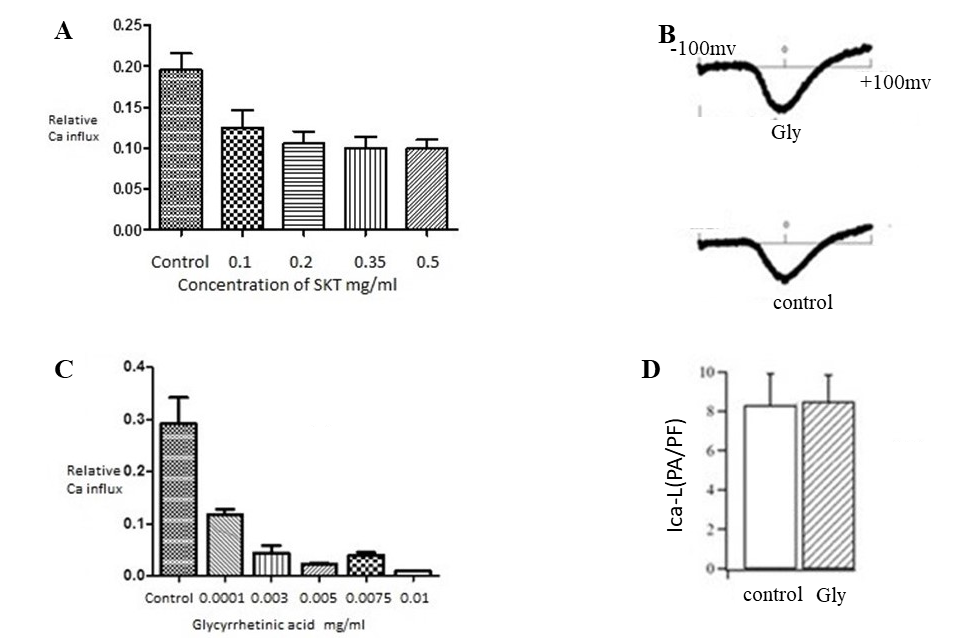
\includegraphics[width=0.8\linewidth]{figure02}
\caption{Fluorescence imaging obtained for actions of SKT (A) and Glycyrrhetinic acid (B) on the pore-forming subunit of the L-type calcium channel expressed in Human Embryonic Kidney (HEK) cells. The dose-response relations were obtained by subtracting calcium imaging levels in conditions when the channels are completely closed from levels when the channels are fully or partly open. The right hand panel shows that experiments using patch clamp recordings at constant voltage do not show the reduced calcium influx. (C): examples of patch clamp recordings. (D): bar plot showing no statistically significant reduction in calcium current. From \citep{noble2016action}.}
\label{fig02}
\end{figure}

\textbf{Validation of the extended model, in which sarcolemmal calcium transporters are incorporated}\\\newline
For validation of the extended model, we used the data on the actions of SKT shown in Figures \ref{fig01} and \ref{fig02}. We tested whether the extended model can reproduce the dynamics of actions of SKT when the L-type calcium channel is blocked by 80\%, to correspond to the maximum block of calcium influx observed in experiments with the pure chemical GA (\autoref{fig02}, right).\\\newpage
The result shows a simple exponential decline in SR calcium, free intracellular calcium and the contraction (\autoref{fig03}). The time constant of decline of the contraction was 22.2 minutes. This is very similar to the experimentally observed time constant of decline in contraction by 10 mg/ml SKT: around 21 minutes in Figure 1. The correspondence between the experimental and model results is very close. Therefore, the extended model succeeds in reproducing the dynamics of SKT when calcium influx is blocked by 80\%. 
The simulation file \href{http://models.cellml.org/workspace/5f4/file/2807f4098d7bfb04507e1d2f876e30aa001e8ead/Fig03.sedml}{Fig03.sedml} contains the computational setting for running the model.
\newline

\begin{figure}[h!]
\centering
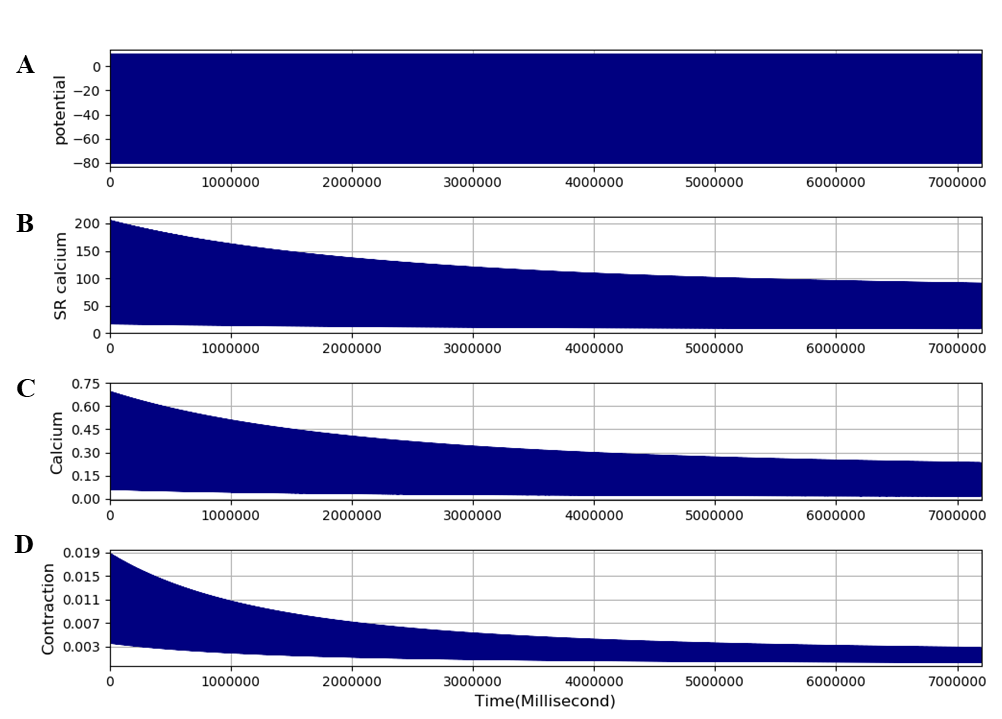
\includegraphics[width=0.9\linewidth]{figure03}
\caption{The extended model was run for 2 hours to reconstruct the dynamics of action of SKT of an 80\% block of ICaL on muscle contraction. 
The traces are: A - membrane potential, B - SR calcium, C - free intracellular calcium, and - contraction. The results presented in this figure can be reproduced with the \href{https://models.physiomeproject.org/workspace/5f4/file/26289d9227fbf4f66ca8106d8bf80ff9a51a5ac6/Fig03.sedml}{Fig03.sedml}}
\label{fig03}
\end{figure}

\textit{Sensitivity Analysis}\\\newline
It is important to determine how robust the extended model is. We carried out sensitivity analysis by increasing all the calcium regulatory network parameters by 50\%, to test the sensitivity of the extended model to likely experimental variations in parameters. The results show that the extended model is robust. No changes in dynamics were greater than the change in parameter (\autoref{fig04}). The correspondence between the experimental and the extended model results for the dynamics of contraction change following block of ICaL is therefore reliable. It is important to note that, apart from adding surface membrane transporters for calcium, we made no other changes to the original model.\newline
\begin{figure}[h!]
\centering
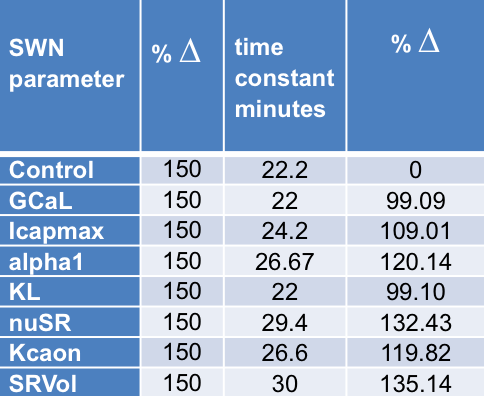
\includegraphics[width=0.43\linewidth]{figure04}
\caption{Results of sensitivity analysis of the extended model \citep{Noble2019Incorporation}.  Each calcium regulatory parameter was increased by 50\%. Changes in the time constant were always less than 50\%.}
\label{fig04}
\end{figure}
\textbf{Experiments in silico}\\\newline
\textit{Comparison of the extended and original models and reconstruction of muscle cramp.}\\\newline
The extended model can therefore be used to perform further experiments, to explore the possible reproduction of muscle cramp. First, we ran the extended model for 100 s at a stimulation frequency of 100 Hz, which produces a tetanic contraction that rapidly declines (fatigue), as illustrated by \autoref{fig05}. The simulation file \href{http://models.cellml.org/workspace/5f4/file/4071d5b4ec40c5e2b845a7a75e942df1966d2ba2/Fig05.sedml}{Fig05.sedml} contains the computational setting for running the model.\newpage

\begin{figure}[h!]
\centering
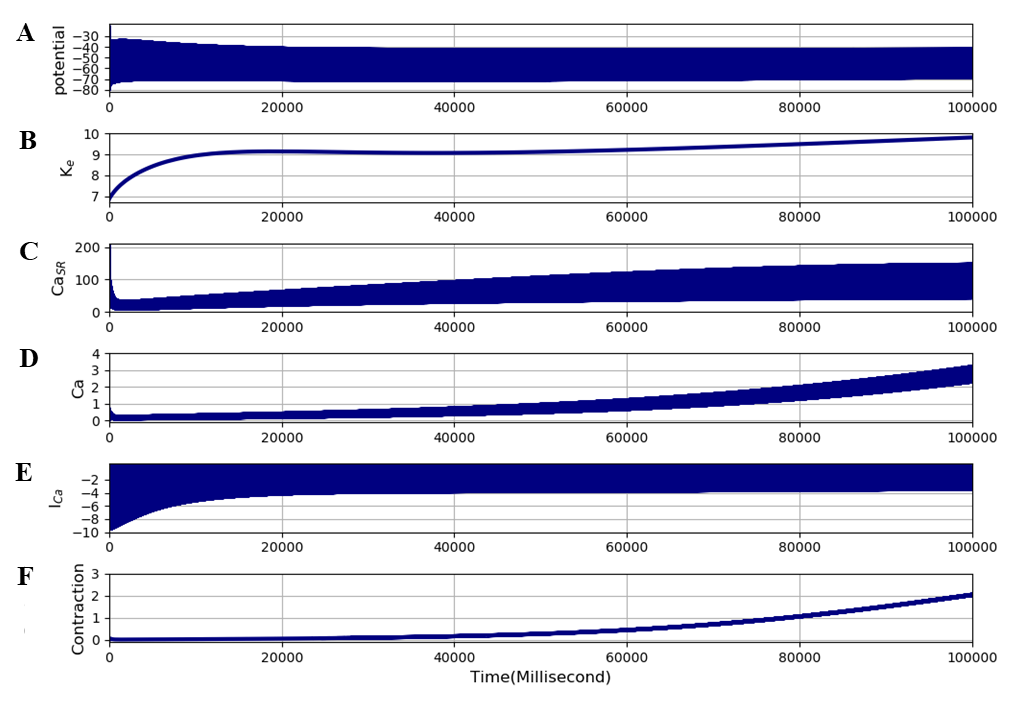
\includegraphics[width=0.9\linewidth]{figure05}
\caption{The extended model was run for 100 seconds at a stimulation frequency of 100 Hz to produce tetanic contractions leading rapidly to fatigue. The traces are: A - membrane potential, B - interstitial potassium, C - SR calcium, D - free intracellular calcium, E - L-type calcium current, and F - contraction (cross-bridge reaction). Note that the slow rise in contraction (actually cross-bridge reaction rate) is so large that the initial response appears very small. The rapid fatigue process is more clearly visible in the contraction panel of \autoref{fig06}. The results presented in this figure can be reproduced with the \href{https://models.physiomeproject.org/workspace/5f4/file/26289d9227fbf4f66ca8106d8bf80ff9a51a5ac6/Fig05.sedml}{Fig05.sedml}}
\label{fig05}
\end{figure}

Prediction by modelling experiments:
\renewcommand{\labelenumi}{(\alph{enumi})}
\begin{enumerate}
     \item accumulation of interstitial potassium, rising to nearly 10 mM. This magnitude of increase in muscle interstitial potassium has been recorded experimentally in human subjects during strong contractions \citep{green2000interstitial} 
     \item gradual rise in SR calcium and calcium release
     \item gradual rise in free intracellular calcium.
     \item calcium-dependent inactivation of ICaL.
     \item large and gradual increase in contraction (rate of cross-bridge reaction).
\end{enumerate}\\ 
Thus, the increase in contraction follows the increase in free intracellular calcium in time course, as shown in figure (c) and (e). Two questions then arise. First, how does this result differ from that of the original unextended model? To answer this question, we repeated the experiment using the same stimulation protocol as in \autoref{fig05}, but with ICaL completely blocked, corresponding to the fact that the original \citep{shorten2007mathematical} model has no ICaL.  The result is shown in \autoref{fig06}. It is clear that the slow rise in free intracellular calcium and in contraction no longer occurs. The simulation file \href{http://models.cellml.org/workspace/5f4/file/4071d5b4ec40c5e2b845a7a75e942df1966d2ba2/Fig06.sedml}{Fig06.sedml} contains the computational setting for running the model. The simulation conditions are exactly same as the one in \autoref{fig05}.
\begin{figure}[h!]
\centering
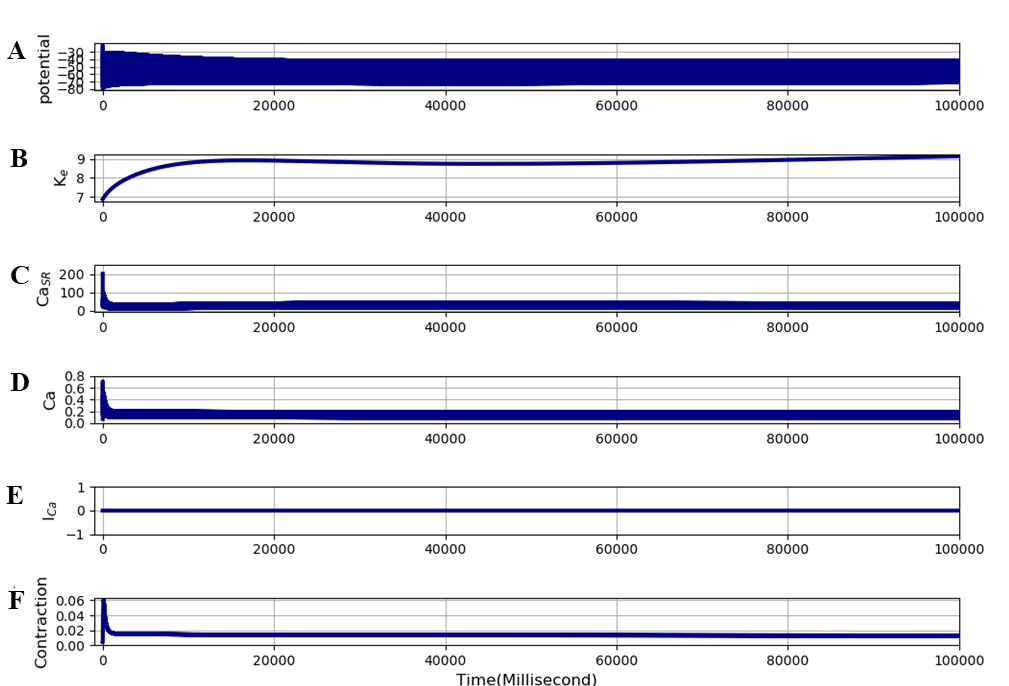
\includegraphics[width=0.9\linewidth]{figure06}
\caption{The extended model was run for 100 seconds at a stimulation frequency of 100 Hz to produce tetanic contractions leading rapidly to fatigue. The only difference from Figure 5 is that ICaL was completely blocked. 
The traces are: A - membrane potential, B - interstitial potassium, C - SR calcium, D - free intracellular calcium, E - L-type calcium current, and F - contraction (cross-bridge reaction). The results presented in this figure can be reproduced with the \href{https://models.physiomeproject.org/workspace/5f4/file/26289d9227fbf4f66ca8106d8bf80ff9a51a5ac6/Fig06.sedml}{Fig06.sedml}}
\label{fig06}
\end{figure}

\begin{figure}[h!]
\centering
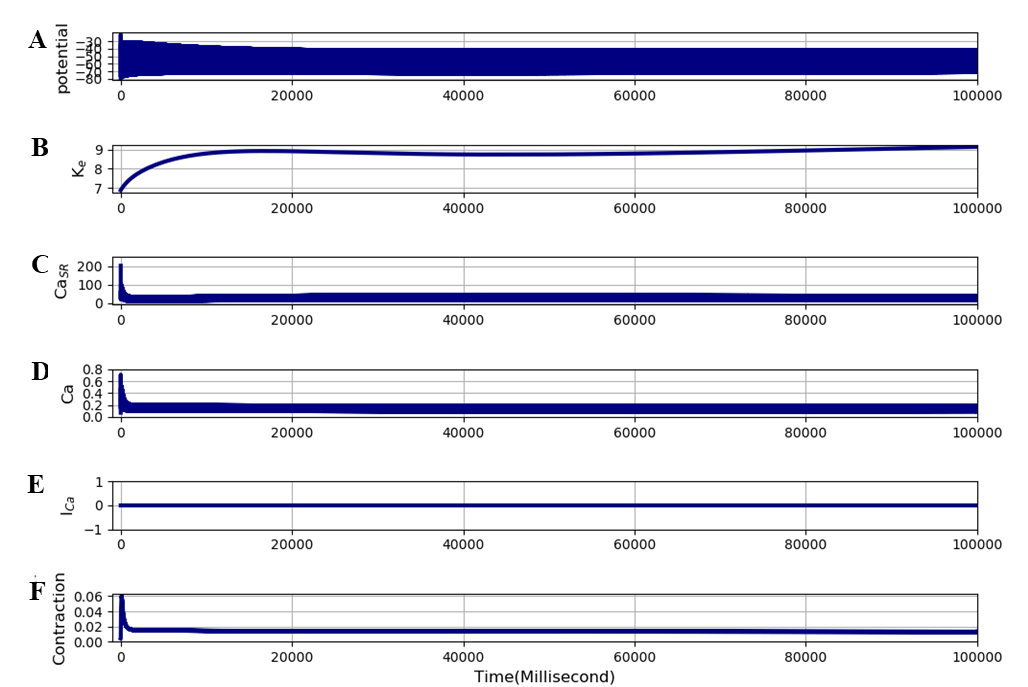
\includegraphics[width=0.9\linewidth]{figure06new}
\caption{Same as \autoref{fig06} except that all surface calcium transporters were set to zero which is similar to original Shorten model. The traces are: A - membrane potential, B - interstitial potassium, C - SR calcium, D - free intracellular calcium, E - L-type calcium current, and F - contraction (cross-bridge reaction). The results presented in this figure can be reproduced with the \href{https://models.physiomeproject.org/workspace/5f4/file/26289d9227fbf4f66ca8106d8bf80ff9a51a5ac6/Fig07.sedml}{Fig07.sedml}}
\label{fig06new}
\end{figure}

We have also calculated the effect of reducing all surface calcium transporters to zero so that only the transporters in the original Shorten model are present. This is important since other calcium transporters, in addition to ICaL, were incorporated into the extended model. This is as expected since ICaL is responsible for nearly all calcium influx. The result is shown in \autoref{fig06new}, which is identical to \autoref{fig06}. As in \autoref{fig06} there is no development of cramp. The simulation file \href{http://models.cellml.org/workspace/5f4/file/4071d5b4ec40c5e2b845a7a75e942df1966d2ba2/Fig07.sedml}{Fig07.sedml} contains the computational setting for running the model. The second question is whether the large slow rise in contraction could represent the cramp process? To answer that question, we performed the same experiment as in \autoref{fig05}, but switched the stimulus off after 100 seconds. To satisfy the definition of cramp, the contraction should not be entirely reversible when the stimuli cease. The result is shown in \autoref{fig07}. At 100 seconds, the magnitude of the contraction in the extended model rapidly drops, but the highly contracted state is not immediately reversible. The rapid drop is attributable to re-uptake by the SR (third trace). The contraction that remains, however, is still very large. It is around 0.5 units, which is 5 times larger than the peak tetanic contraction (0.1 units) before fatigue in \autoref{fig06}. This remaining strong contraction then slowly declines. Thus, the result in \autoref{fig07} does reproduce the state of cramp. The simulation file \href{http://models.cellml.org/workspace/5f4/file/4071d5b4ec40c5e2b845a7a75e942df1966d2ba2/Fig08.sedml}{Fig08.sedml} contains the computational setting for running the model.

\begin{figure}[h!]
\centering
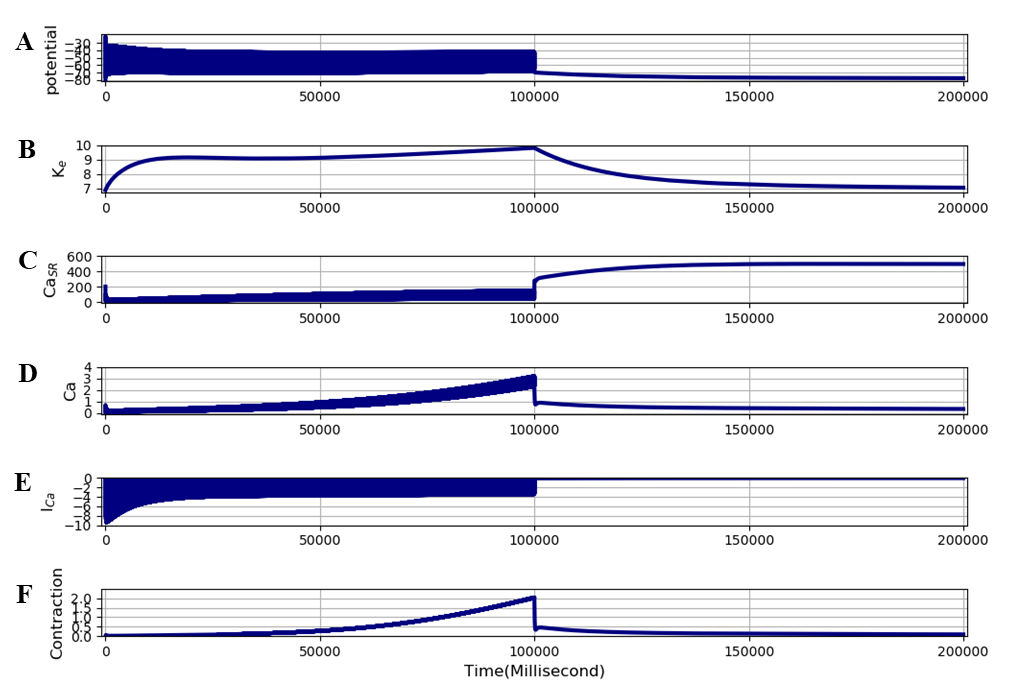
\includegraphics[width=0.9\linewidth]{figure07}
\caption{The extended model was run for 200 seconds at a stimulation frequency of 100 Hz to produce tetanic contractions leading rapidly to fatigue. The stimuli were then stopped after 100 seconds. The traces are: A - membrane potential, B - interstitial potassium, C - SR calcium, D - free intracellular calcium, E - calcium current (ICaL), F - and contraction (cross-bridge reaction). The results presented in this figure can be reproduced with the \href{https://models.physiomeproject.org/workspace/5f4/file/26289d9227fbf4f66ca8106d8bf80ff9a51a5ac6/Fig08.sedml}{Fig08.sedml}}
\label{fig07}
\end{figure}

\begin{figure}[h!]
\centering
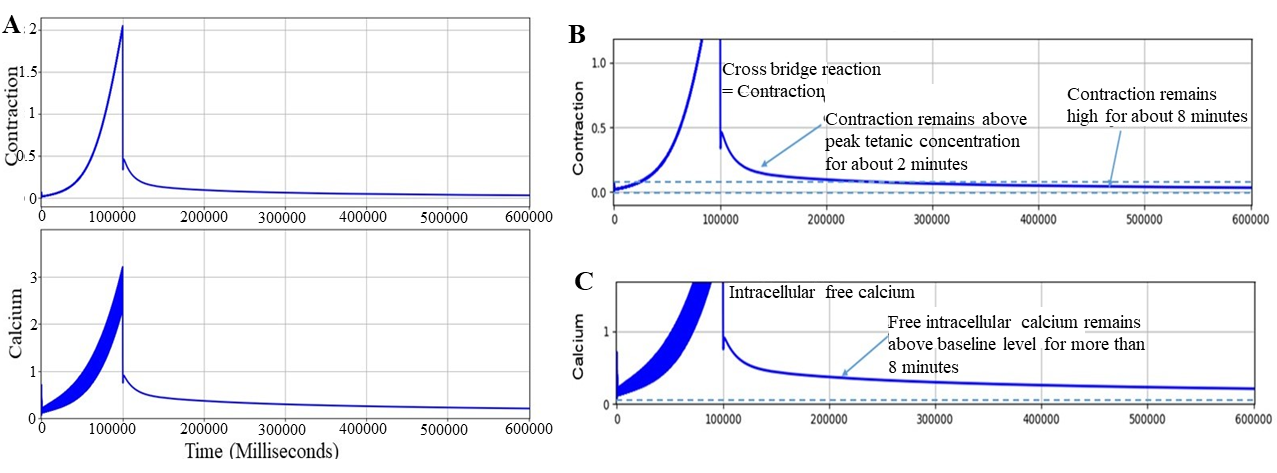
\includegraphics[width=1\linewidth]{figure8-}
\caption{A - The extended model was run for 600 seconds at a stimulation frequency of 100 Hz to produce tetanic contractions leading rapidly to fatigue. The stimuli were then stopped after 100 seconds. 
B - Lower part of contraction. C - Lower part of free intracellular calcium. The results presented in this figure can be reproduced with the \href{https://models.physiomeproject.org/workspace/5f4/file/26289d9227fbf4f66ca8106d8bf80ff9a51a5ac6/Fig09.sedml}{Fig09.sedml}}
\label{fig08}
\end{figure}\newpage

Lower frequencies of stimulation produced small degrees of calcium accumulation. By the definition of cramp we are using, frequencies of 25 Hz and lower did not produce the cramped state. We have therefore used 100 Hz as standard, which readily produced cramp and permits computational experiments on possible mechanisms of reversal. \autoref{fig08} shows the result of a 10-minute run showing the free intracellular calcium and contraction on higher scales. The free intracellular calcium remains high throughout the run. The contraction remains above peak tetanic contraction for about 2 minutes, and remains high for about 8 minutes. By the usual criterion defining the condition of cramp, the results in Figures \ref{fig07} and \ref{fig08} show that the extended model automatically produces a model of cramp. The important discovery is that calcium influx is essential for producing cramp, as shown in Figures \ref{fig06}, \ref{fig07} and \ref{fig08}. The simulation file \href{http://models.cellml.org/workspace/5f4/file/4071d5b4ec40c5e2b845a7a75e942df1966d2ba2/Fig09.sedml}{Fig09.sedml} contains the computational setting for running the model.

\title{\textit{Reversal of the cramp condition}}\\\newline
The comparison between Figures \ref{fig05} and \ref{fig06} shows that reducing calcium influx would be expected to delay or prevent cramp. But, how could cramp be reversed, once the cramped state has developed? To answer this question we performed the computational experiments shown in Figures \ref{fig09}-\ref{fig11}.\\\newline

\begin{figure}[h!]
\centering
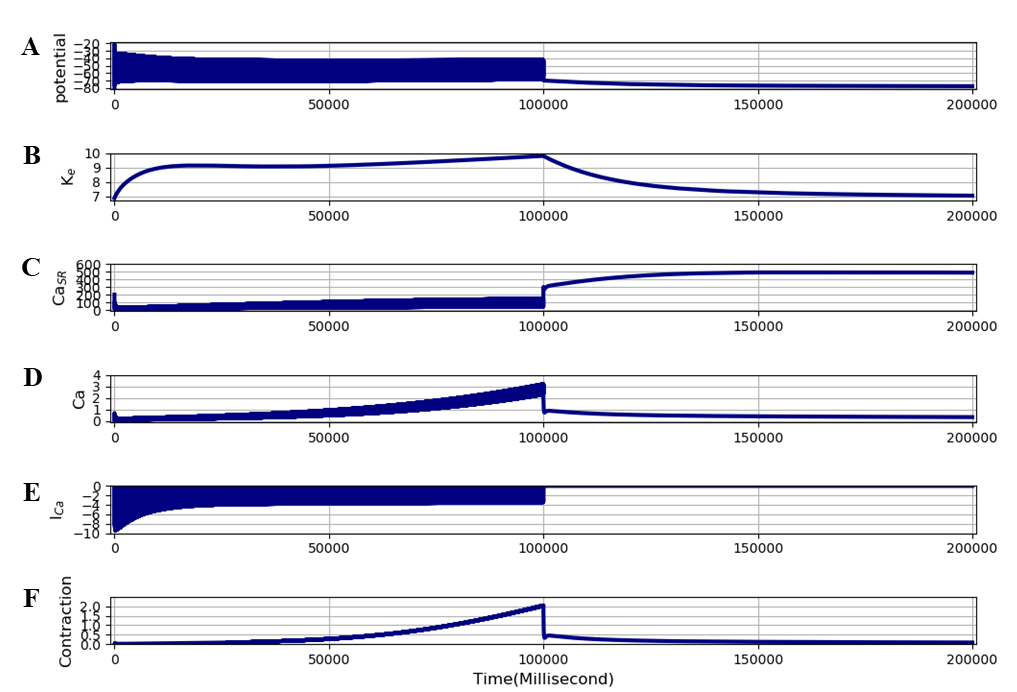
\includegraphics[width=0.9\linewidth]{figure09}
\caption{This computational experiment uses the same protocol as Figure 7 except that the L-type calcium channel was blocked after stimuli were stopped (i.e. after 100 seconds). The traces are: A - membrane potential, B - interstitial potassium, C - SR calcium, D - free intracellular calcium, E - calcium current (ICaL), F - and contraction (cross-bridge reaction). The results presented in this figure can be reproduced with the \href{https://models.physiomeproject.org/workspace/5f4/file/26289d9227fbf4f66ca8106d8bf80ff9a51a5ac6/Fig10.sedml}{Fig10.sedml}}
\label{fig09}
\end{figure}

\autoref{fig09} uses the same protocol as \autoref{fig07}, except that ICaL was blocked at the time at which stimulation ceased. The result shows that the strong maintained contraction (cramp state) persists for the same period of time as in \autoref{fig07}. The simulation file \href{http://models.cellml.org/workspace/5f4/file/4071d5b4ec40c5e2b845a7a75e942df1966d2ba2/Fig10.sedml}{Fig10.sedml} contains the computational setting for running the model. The simulation conditions are exactly same as the one in \autoref{fig07}.\newline 
The comparison between the results in Figures \ref{fig07} and \ref{fig09} shows that block of ICaL does not reverse the cramped state once it has developed.Because calcium influx is essential in the model for creating the cramp condition, it is reasonable to think that calcium efflux must be a necessary component of its reversal. We therefore performed computational experiments to explore the possible mechanisms that could produce sufficient calcium efflux for reversing the cramp state. We found that the extended model successfully reproduces the process of reversing cramp, provided that the accumulation of potassium is rapidly reversed. As we showed in the other paper \citep{Noble2019Incorporation} the extended model includes this process.\newpage
\begin{figure}[h!]
\centering
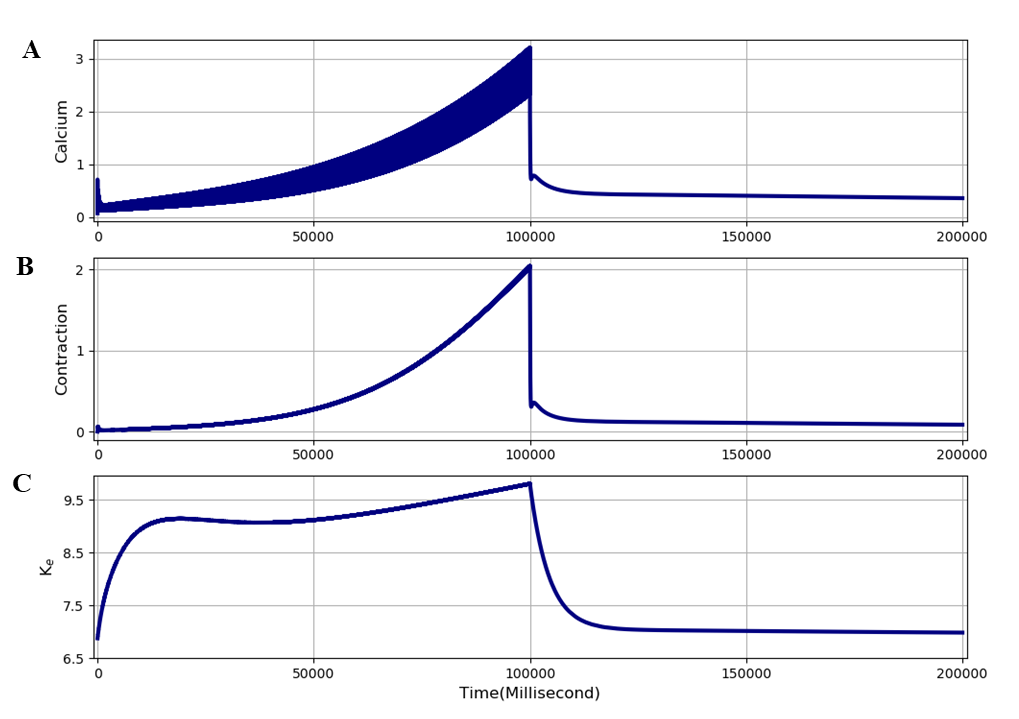
\includegraphics[width=0.9\linewidth]{figure10}
\caption{Result of a computational experiment using extended model, in which rapid wash-out is mimicked by reducing plasma potassium concentration and decreasing the time constant for exchange between plasma, interstitial and tubular potassium concentrations. A - Free intracellular calcium, B - Contraction, C - Interstitial potassium. The results presented in this figure can be reproduced with the \href{https://models.physiomeproject.org/workspace/5f4/file/26289d9227fbf4f66ca8106d8bf80ff9a51a5ac6/Fig11.sedml}{Fig11.sedml}}
\label{fig10}
\end{figure}

The result is shown in \autoref{fig10}. The protocol was the same as in Figures \ref{fig07} and \ref{fig09} up to the point where simulation was ceased (i.e. after 100 seconds). At that point:
\renewcommand{\labelenumi}{(\alph{enumi})}
\begin{enumerate}
     \item the bulk extracellular potassium concentration was reduced to an assumed normal plasma level (4 mM). 
     \item the time constants of exchange with bulk potassium and between tubular and interstitial potassium were reduced to 20\% of their standard values to mimic rapid wash-out via increased blood flow.
\end{enumerate}\\\newline 
The result in \autoref{fig10} shows a rapid wash-out of the accumulated potassium, which is almost complete within 20 seconds. The cramp state is completely reversed within around 10 seconds. Wash-out of potassium is sufficient to reverse cramp condition. The simulation file \href{http://models.cellml.org/workspace/5f4/file/099d70c2ee6ed5dfb1ca33e0ce16db4f0247a4dc/Fig11.sedml}{Fig11.sedml} contains the computational setting for running the model.\\


\title{\textit{Superimposition of the cramped and relieved states}}\newline


\autoref{fig11} shows superimposition of the contraction traces from the results illustrated in Figures \ref{fig09} and \ref{fig10}. Without potassium wash-out, the cramp state persists for at least 2 minutes. With potassium wash-out, the cramp state disappears within 10 seconds. In order to investigate the interactions between the processes involved, we performed computational experiments on an expanded time scale, as shown in Figures \ref{fig12} and \ref{fig13}. \autoref{fig12} shows a more complete set of traces obtained on a larger time scale by calculating the changes occurring during the first 20 seconds of the simulation in \autoref{fig09} following cessation of stimulation. The expanded time scale in \autoref{fig12} enables us to investigate the interactions between the processes involved. Calcium efflux following potassium wash-out occurs through activation of sodium-calcium exchange.\\

\begin{figure}[h!]
\centering
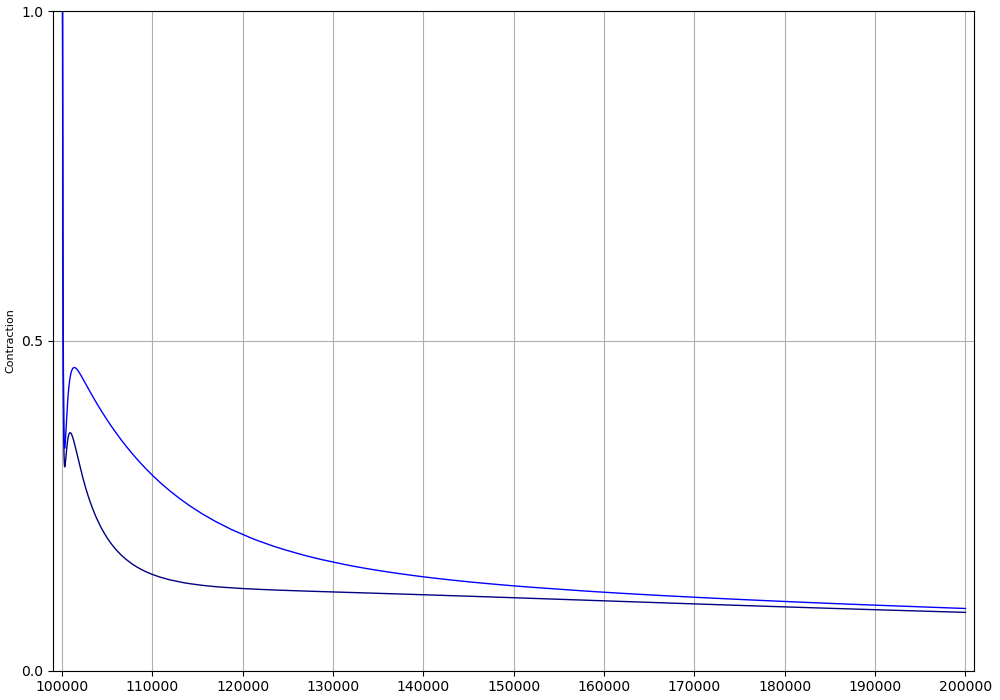
\includegraphics[width=0.8\linewidth]{figure11}
\caption{Superimposed traces of the decline in force of contraction (cross-bridge reaction) following cessation of stimulation, and with and without potassium wash-out. Without wash-out, contraction remains above peak tetanic contraction for nearly 2 minutes. With wash-out, the model shows complete relaxation to the baseline within 10 seconds. The results presented in this figure can be reproduced with the \href{https://models.physiomeproject.org/workspace/5f4/file/26289d9227fbf4f66ca8106d8bf80ff9a51a5ac6/Fig12.sedml}{Fig12.sedml}}
\label{fig11}
\end{figure}



The simulation file \href{http://models.cellml.org/workspace/5f4/file/4071d5b4ec40c5e2b845a7a75e942df1966d2ba2/Fig13.sedml}{Fig13.sedml} contains the computational setting for running the model. After 10 seconds after the simulation is stopped and values are changed, simulation results were cleared and the ending point was changed to 20000 milliseconds and all the stimulation was removed, finally simulation was run again for 20 seconds.\newline


The results in \autoref{fig13} shows that the fall of free intracellular calcium (fourth trace) is largely produced by activation of sodium-calcium exchange (bottom trace). The top two traces in \autoref{fig13} show that the change in membrane potential in a hyperpolarizing direction closely follows the change in interstitial potassium, as expected since the resting potential is largely determined by the Nernst equation for potassium ions. Free intracellular calcium (fourth trace) initially falls very rapidly. The simulation file \href{http://models.cellml.org/workspace/5f4/file/4071d5b4ec40c5e2b845a7a75e942df1966d2ba2/Fig14.sedml}{Fig14.sedml} contains the computational setting for running the model. The simulation conditions are exactly same as the one in \autoref{fig12}.

\begin{figure}[h!]
\centering
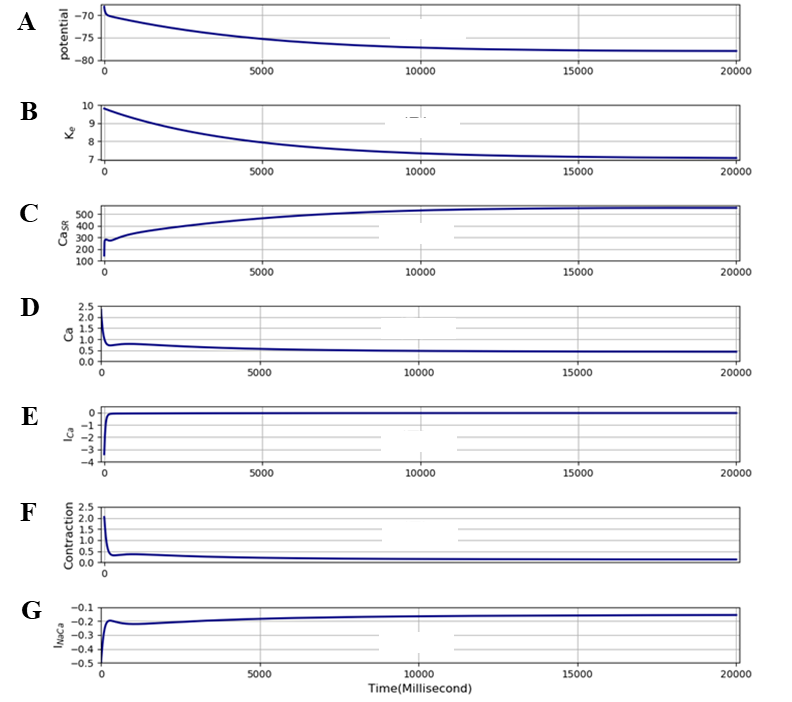
\includegraphics[width=0.7\linewidth]{figure12}
\caption{This shows changes in A - membrane potential, B - interstitial potassium, C - SR calcium, D - free intracellular calcium, E - L-type calcium current , F - contraction and G - the sodium-calcium exchange current during the first 20 seconds after stimulation ceases in the computation illustrated in \autoref{fig10}. The results presented in this figure can be reproduced with the \href{https://models.physiomeproject.org/workspace/5f4/file/26289d9227fbf4f66ca8106d8bf80ff9a51a5ac6/Fig13.sedml}{Fig13.sedml}}
\label{fig12}
\end{figure}

\begin{figure}[h!]
\centering
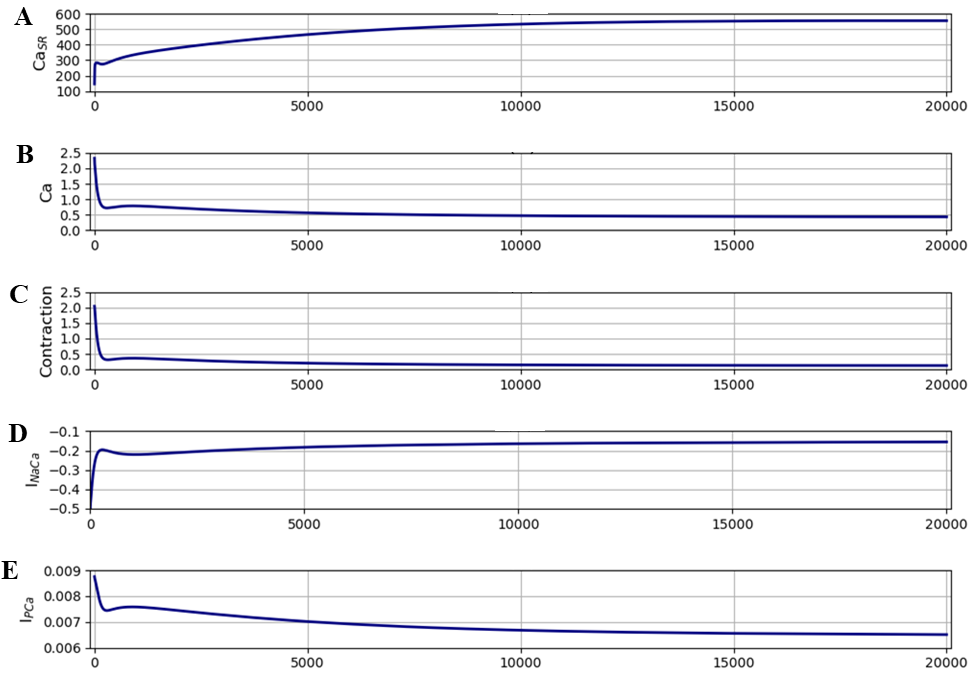
\includegraphics[width=0.8\linewidth]{figure13}
\caption{This shows changes in A - SR calcium, B - free intracellular calcium, C - Contraction, D - the sodium-calcium exchange current, E - the calcium pump current during the first 20 seconds after stimulation ceases in the computation illustrated in Figure. The results presented in this figure can be reproduced with the \href{https://models.physiomeproject.org/workspace/5f4/file/26289d9227fbf4f66ca8106d8bf80ff9a51a5ac6/Fig14.sedml}{Fig14.sedml}}\newpage
\label{fig13}
\end{figure}

The changes are shown on a larger time scale in \autoref{fig13}, where we have also included the changes in the calcium pump current, which plays a relatively minor role in the model. The middle trace (contraction) in \autoref{fig13} shows that there are two phases of fall in contraction in the model. The first, rapid, phase lasts about 200 milliseconds and is largely driven by the fall in free intracellular calcium produced by the high activity of the sodium-calcium exchange. This phase corresponds to the time taken to remove the calcium overload. Free intracellular calcium falls towards the usual maximum level during contraction, i.e. around 1 µM.  There is then a slower phase of recovery driven by both the sodium-calcium exchange and the calcium pump.\\\newline
The computations shown in Figures \ref{fig05}-\ref{fig12} were all performed with the time constant (TauK3) for exchange between interstitial [K]$_e$ and bulk [K]$_b$ set to a standard value, which was arbitrarily set to the value of the time constant for exchange between tubular and interstitial potassium in the original \citep{shorten2007mathematical} model, i.e.TauK2. Given the greater distances that must be involved in the exchange with [K]$_b$, the time constant for exchange with bulk potassium must actually be larger than TauK2. Moreover, in a cramped muscle, circulation will be reduced. We therefore performed calculations with TauK3 set to 200 seconds to represent such a situation (\autoref{fig14}). There are several important outcomes of this experiment:
\renewcommand{\labelenumi}{(\alph{enumi})}
\begin{enumerate}
     \item a shorter period of stimulation (60 seconds) was needed to model the cramp process.
     \item accumulation of interstitial potassium was greater and so was the magnitude of the cramped state as a result.
     \item the contraction, after stimulation stopped, decayed more slowly and lasted much longer.
     \item when potassium wash-out was induced by reducing TauK3 to 4 seconds, the cramp state was relieved very rapidly. 
\end{enumerate}\newline

\begin{figure}[h!]
\centering
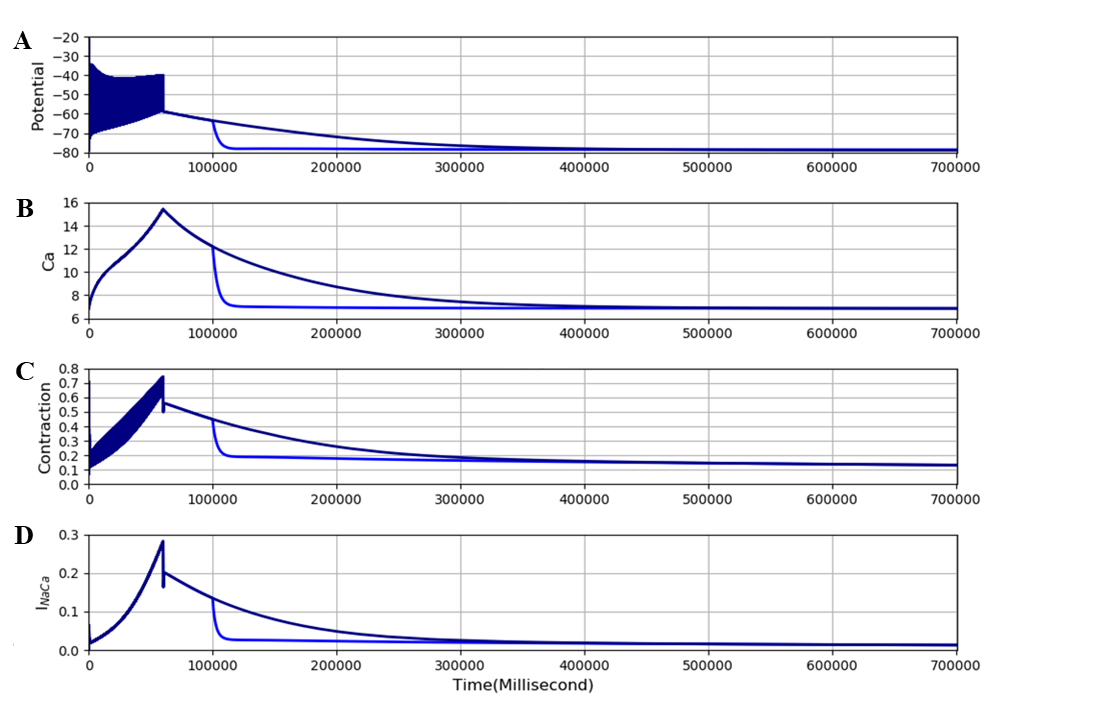
\includegraphics[width=0.9\linewidth]{figure14}
\caption{Result of an experiment lasting 700 seconds when TauK3 is increased approximately ten fold to 200 seconds. The extended model was stimulated at 100 Hz for 60 seconds. This produces a much longer period of cramp. The large contraction when stimulation stops is then maintained for a longer period of time. The figures shows superimposition of an experiment in which the slow exchange between [K]e and [K]b was maintained, and one in which just after 100 seconds, TauK3 was reduced to 4 seconds to produce rapid wash-out of potassium. The results presented in this figure can be reproduced with the \href{https://models.physiomeproject.org/workspace/5f4/file/26289d9227fbf4f66ca8106d8bf80ff9a51a5ac6/Fig15(01).sedml}{Fig15(01) and \href{https://models.physiomeproject.org/workspace/5f4/file/26289d9227fbf4f66ca8106d8bf80ff9a51a5ac6/Fig15(02).sedml}{Fig15(02)}}}
\label{fig14}
\end{figure}\newline

It is noteworthy, however, that the increase in duration of the maintained contraction after stimulation ceases (about 3 fold) is not as long as the increase in time constant (about 10 fold). Another process must therefore be contributing to reducing interstitial potassium. The simulation files \href{http://models.cellml.org/workspace/5f4/file/099d70c2ee6ed5dfb1ca33e0ce16db4f0247a4dc/Fig15(01).sedml}{Fig15(01).sedml} and \href{http://models.cellml.org/workspace/5f4/file/099d70c2ee6ed5dfb1ca33e0ce16db4f0247a4dc/Fig15(02).sedml}{Fig15(02).sedml}contain the computational setting for running the model.\\


As noted in the other paper \citep{Noble2019Incorporation}, the initial steady state contraction in the extended model is very low compared to the original model. In that paper, we outlined how that deficiency might be rectified in future re-parameterisation of the extended model. In particular, we showed that increasing the calcium uptake rate, nuSR, into the SR can readily increase steady state contraction.\newpage 

\begin{figure}[h!]
\centering
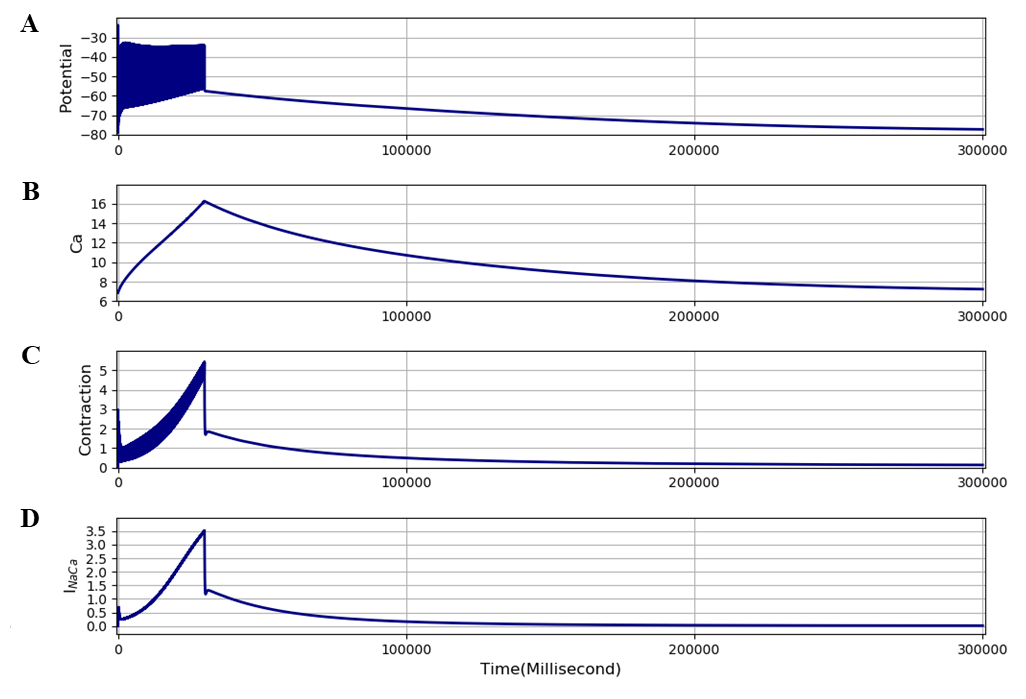
\includegraphics[width=0.9\linewidth]{figure15}
\caption{Result obtained with the extended model adjusted to produce a larger steady state contraction by increasing nuSR to15 (about 3 times the value used in the original model). The model was stimulated at 100 Hz for 30 seconds. The results presented in this figure can be reproduced with the \href{https://models.physiomeproject.org/workspace/5f4/file/26289d9227fbf4f66ca8106d8bf80ff9a51a5ac6/Fig16.sedml}{Fig16.sedml}}
\label{fig15}
\end{figure}


\newpage
We have therefore also run computations with the nuSR parameter increased to 15 and 35. Both levels of nuSR produce much larger steady state contractions, as shown in \autoref{fig06new} of the other paper \citep{Noble2019Incorporation}, but the development of the maintained (cramp) condition still occurs, as shown in \autoref{fig15}. The level of maintained contraction is much larger than in \autoref{fig14}, 1.25 compared to 0.35, but decays faster. The faster decay is attributable to a larger activation of the sodium-calcium exchange current by larger intracellular contraction. The simulation file \href{http://models.cellml.org/workspace/5f4/file/099d70c2ee6ed5dfb1ca33e0ce16db4f0247a4dc/Fig16.sedml}{Fig16.sedml} contains the computational setting for running the model. The value of TauK3 was set to 200 seconds. The interplays between the various parameter adjustments that can restore larger steady state contractions in the model are complex and would require further investigation of the parameter spaces involved in future work.

\section{Discussion}

\textit{Significance of sarcolemmal calcium fluxes in skeletal muscle}\\\newline
Sarcolemmal calcium influx is not necessary for individual twitch responses in skeletal muscle since the trigger for electromechanical coupling is entirely electrical. This property is what enabled \cite{shorten2007mathematical} to reproduce contraction and fatigue in their model with only intracellular recycling of calcium.\\\newline 
However, by adding equations for the sarcolemmal calcium fluxes, we have shown that over periods of time greater than a few tens of seconds the sarcolemmal calcium fluxes would be expected to have a significant effect on intracellular calcium concentrations and therefore on electromechanical coupling. We show in this paper that these small fluxes do gradually alter SR calcium and intracellular free calcium. The slow time course of those changes closely corresponds to the dynamics of change in contraction observed experimentally when a medication that reduces calcium influx is used. This close correspondence with experimental data partially validates the model.\\\newline
\textit{Significance of calcium efflux, conditions for cramp, its prevention, and its reversal}\\\newline
One of the aims of our extension of the model is to reproduce cramp. We define cramp to be a maintained contraction that continues for a substantial period of time without stimulation and is therefore initially not reversible by nervous control.\\\newline 
The model satisfies this condition. Even though small on a beat-to-beat time scale, the increased calcium influx at high frequencies is predicted to be sufficient to produce calcium overload to generate a cramped state. The extended model is thus the first successful mathematical model of skeletal muscle cramp. It is useful as a model for the study of cramp induced by vigorous exercise. However, it remains to be seen whether rest cramps might also be reproduced by the model. A possible clue from our work is the facilitation and maintenance of cramp by increased interstitial potassium. If rest cramps are produced through poor circulation, leading to accumulation of interstitial potassium, then they might have a common mechanism. That question remains to be answered.\\\newline
We show that the model also makes an important prediction on how cramp may be relieved rapidly. The prediction is that wash-out of interstitial potassium is necessary to relieve the cramp process. Effectively, high interstitial potassium maintains the cramped state. Relief depends on increased calcium efflux via the sodium-calcium exchange led by the wash-out of interstitial potassium. The model therefore indicates that a mechanism that relieves cramp must improve the circulation through vasodilation, so achieving wash-out of interstitial potassium. All these predictions are experimentally testable.\\\newline
The result shown in \autoref{fig13} implies that another process must also be contributing to removing interstitial potassium. In the extended model, the only process that can do this is the sodium-potassium (Na$^+$,K$^+$-ATPase) pump, which generates potassium influx in exchange for sodium efflux. This interpretation is strongly supported by \citep{nielsen2004effects} who showed the effect of high-intensity training on the kinetics of interstitial potassium changes in human subjects. Training increases the activity of the Na$^+$,K$^+$-ATPase pumps and reduces the interstitial potassium accumulation during exercise. \\\newline
Of course, it will require further investigations of the extended model to clarify the conditions under which this process develops and how it recovers. These model investigations would best be done in conjunction with human experiments on cramp following vigorous exercise, and to compare the model predictions with experimental recordings of biochemical parameters during vigorous exercise. \\\newline
\textit{Further discussion from an evolutionary perspective}\\\newline
Our results also have implications for the evolution of skeletal muscle in having become so different from smooth and cardiac muscle in the role of calcium influx. Very low levels of calcium influx in skeletal muscle could be seen to be adaptive since high levels of calcium influx would generate the cramp mechanism too rapidly during maintained tetanic contractions. It is significant that we needed to use high-frequency stimulation to generate the cramp state.\\\newline
\textbf{Acknowledgements.} We express our gratitude to TSUMURA \& CO. for funding the “University of Oxford Innovative Systems Biology Project sponsored by Tsumura”. We acknowledge the following laboratories where some of the experimental work was done: Laboratory of Professor Derek Terrar at the Department of Pharmacology, University of Oxford (Figure 1); Laboratory of Professor Anant Parekh at the Department of Physiology, Anatomy and Genetics, Oxford University (Figure 2).\newpage

\bibliography{References}

\end{document}